\chapter*{Dodatak: Prikaz aktivnosti grupe}
		\addcontentsline{toc}{chapter}{Dodatak: Prikaz aktivnosti grupe}
		
		\section*{Dnevnik sastajanja}
		
		%\textbf{\textit{Kontinuirano osvježavanje}}\\
		
		% \textit{U ovom dijelu potrebno je redovito osvježavati dnevnik sastajanja prema predlošku.}
		
		\begin{packed_enum}
			\item  sastanak
			
			\item[] \begin{packed_item}
				\item Datum: u ovom formatu: 20.10.2022.
				\item Prisustvovali: J.Vrsalović, V.Krušić, A.Macan, P.Novak, V.Perković, L.Vrsalović, L.Zekan
				\item Teme sastanka:
				\begin{packed_item}
					\item  ideje o dodijeljenoj temi
					\item  raspodjela uloga u timu
				\end{packed_item}
			\end{packed_item}
			
			\item  sastanak
			\item[] \begin{packed_item}
				\item Datum: u ovom formatu: 26.10.2022.
				\item Prisustvovali: L.Vrsalović, V.Perković
				\item Teme sastanka:
				\begin{packed_item}
					\item  Podjela posla u dokumentaciji
					\item  Instalacija i pokretanje alata
				\end{packed_item}
			\end{packed_item}
			
			\item  sastanak
			\item[] \begin{packed_item}
				\item Datum: u ovom formatu: 2.11.2022.
				\item Prisustvovali: J.Vrsalović, Petar Novak, Anton Macan
				\item Teme sastanka:
				\begin{packed_item}
					\item  Back end
					\item  Koncept baze podataka
				\end{packed_item}
			\end{packed_item}
			
			\item  sastanak
			\item[] \begin{packed_item}
				\item Datum: u ovom formatu: 3.11.2022.
				\item Prisustvovali: J.Vrsalović, V.Krušić, L.Zekan
				\item Teme sastanka:
				\begin{packed_item}
					\item  Login forma
					\item  Homepage
				\end{packed_item}
			\end{packed_item}
			
			\item  sastanak
			\item[] \begin{packed_item}
				\item Datum: u ovom formatu: 5.12.2022.
				\item Prisustvovali: A. Macan, P. Novak
				\item Teme sastanka:
				\begin{packed_item}
					\item  Usklađivanje baze podataka
					\item  Planovi za dalje
				\end{packed_item}
			\end{packed_item}
			
			\item  sastanak
			\item[] \begin{packed_item}
				\item Datum: u ovom formatu: 9.12.2022.
				\item Prisustvovali: J.Vrsalović, V.Krušić, A.Macan, P.Novak, V.Perković, L.Vrsalović, L.Zekan
				\item Teme sastanka:
				\begin{packed_item}
					\item  Tražilica
					\item  Plan za nastavak rada
				\end{packed_item}
			\end{packed_item}
			
			\item  sastanak
			\item[] \begin{packed_item}
				\item Datum: u ovom formatu: 15.12.2022.
				\item Prisustvovali: J.Vrsalović, L.Zekan
				\item Teme sastanka:
				\begin{packed_item}
					\item  Refaktoriranje frontenda
					\item  razni bugovi
				\end{packed_item}
			\end{packed_item}
			
			\item  sastanak
			\item[] \begin{packed_item}
				\item Datum: u ovom formatu: 1.1.2023.
				\item Prisustvovali: J.Vrsalović, L.Zekan, V. Krušić
				\item Teme sastanka:
				\begin{packed_item}
					\item  Frontend
					\item  Oznake na proizvodima
				\end{packed_item}
			\end{packed_item}
			
			\item  sastanak
			\item[] \begin{packed_item}
				\item Datum: u ovom formatu: 1.1.2023.
				\item Prisustvovali: L.Vrsalović, V.Perković
				\item Teme sastanka:
				\begin{packed_item}
					\item  Raspodjela posla dokumentacije
				\end{packed_item}
			\end{packed_item}
			%
			\item  sastanak
			\item[] \begin{packed_item}
				\item Datum: u ovom formatu: 5.1.2023.
				\item Prisustvovali: J.Vrsalović, L.Zekan, P.Novak, A.Macan
				\item Teme sastanka:
				\begin{packed_item}
					\item  Funkcionalnost obavijesti
					\item  Testiranje softvera
				\end{packed_item}
			\end{packed_item}
			
		\end{packed_enum}
		
		\eject
		\section*{Tablica aktivnosti}
		
			%\textbf{\textit{Kontinuirano osvježavanje}}\\
			
			% \textit{Napomena: Doprinose u aktivnostima treba navesti u satima po članovima grupe po aktivnosti.}

			\begin{longtblr}[
					label=none,
				]{
					vlines,hlines,
					width = \textwidth,
					colspec={X[7, l]X[1, c]X[1, c]X[1, c]X[1, c]X[1, c]X[1, c]X[1, c]}, 
					vline{1} = {1}{text=\clap{}},
					hline{1} = {1}{text=\clap{}},
					rowhead = 1,
				} 
				\multicolumn{1}{c|}{} & \multicolumn{1}{c|}{\rotatebox{90}{\textbf{Joško Vrsalović}}} & \multicolumn{1}{c|}{\rotatebox{90}{\textbf{Vida Krušić}}} &	\multicolumn{1}{c|}{\rotatebox{90}{\textbf{Anton Macan }}} & \multicolumn{1}{c|}{\rotatebox{90}{\textbf{Petar Novak }}} &	\multicolumn{1}{c|}{\rotatebox{90}{\textbf{Vlado Perković }}} & \multicolumn{1}{c|}{\rotatebox{90}{\textbf{Lovro Vrsalović }}} &	\multicolumn{1}{c|}{\rotatebox{90}{\textbf{Luka Zekan }}} \\  
				Upravljanje projektom 		& 20 &  &  &  &  &  & \\ 
				Opis projektnog zadatka 	&  &  &  &  & 4 &  & \\ 
				
				Funkcionalni zahtjevi       &  &  &  &  &  & 1 &  \\ 
				Opis pojedinih obrazaca 	&  &  &  &  & 1 & 4 &  \\ 
				Dijagram obrazaca 			&  &  &  &  &  & 3 &  \\ 
				Sekvencijski dijagrami 		&  &  &  &  & 2 &  &  \\ 
				Opis ostalih zahtjeva 		&  &  &  &  &  & 1 &  \\ 

				Arhitektura i dizajn sustava	 &  &  &  &  &  &  & 3 \\ 
				Baza podataka				&  &  & 4 &  &  &  &   \\ 
				Dijagram razreda 			&  &  &  & 5 &  &  &   \\ 
				Dijagram stanja				&  &  &  &  &  & 4 &  \\ 
				Dijagram aktivnosti 		&  &  &  &  &  & 3 &  \\ 
				Dijagram komponenti			&  &  &  &  & 4 &  &  \\ 
				Korištene tehnologije i alati 		&  &  &  &  & 2 &  &  \\ 
				Ispitivanje programskog rješenja 	&  &  & 3 &  & 1 &  &  \\ 
				Dijagram razmještaja			&  &  &  &  & 2 &  &  \\ 
				Upute za puštanje u pogon 		& 1 &  &  &  & 3 &  &  \\  
				Dnevnik sastajanja 			&  &  &  &  & 2 &  &  \\ 
				Zaključak i budući rad 		&  &  &  &  & 2 &  &  \\  
				Popis literature 			&  &  &  &  & 1 &  &  \\  
				&  &  &  &  &  &  &  \\ \hline 
				\textit{homepage} 			&  & 4 &  &  &  &  & 1 \\ 
				\textit{forme za login i signup} 				&  & 2 &  &  &  &  &  \\  
				\textit{izrada baze podataka} 		 			&  &  & 4 &  &  &  & \\  
				\textit{spajanje s bazom podataka} 							&  &  &  & 4 &  &  &  \\ 
				\textit{back end} 							& 2 &  &  & 5 &  &  &  \\  
				\textit{deployment} 			& 7 &  &  &  &  &  &  \\
				&  &  &  &  &  &  &  \\ \hline
				\textit{frontend} 			&  & 4 &  & 1 &  &  & 22 \\
				\textit{backend} 			& 17 &  & 7 & 21 &  &  & 4 \\
			\end{longtblr}
					
					
		\eject
		\section*{Dijagrami pregleda promjena}
		
		%\textbf{\textit{dio 2. revizije}}\\
		
		%\textit{Prenijeti dijagram pregleda promjena nad datotekama projekta. Potrebno je na kraju projekta generirane grafove s gitlaba prenijeti u ovo poglavlje dokumentacije. Dijagrami za vlastiti projekt se mogu preuzeti s gitlab.com stranice, u izborniku Repository, pritiskom na stavku Contributors.}
		
		\begin{figure}[H]
			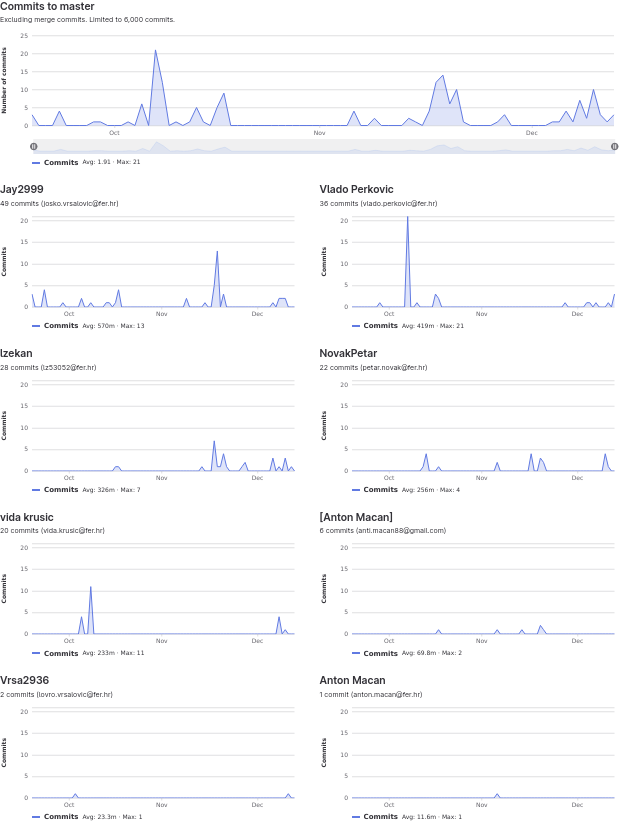
\includegraphics[width=\textwidth]{slike/commitovi.png} %veličina u odnosu na širinu linije
			\caption{Prikaz aktivnosti na repozitoriju}
			\label{fig:commitovi} %label mora biti drugaciji za svaku sliku
			\end{figure}
		
	